\chapter{Prompt Engineering}
\label{ch:prompting}

\epigraph{``Most production AI is prompt engineering. The rest is plumbing.''}{}

This chapter covers \textbf{Section~2: Prompt Engineering (16\% of the exam)}. The exam expects you to write prompts, choose parameters, manage templates, and understand the risks. Every sub-section below maps to an official objective (2.1--2.8). If you have not yet read Chapter~\ref{ch:foundations}, do so first --- model selection (Section~1.5) drives the prompt choices in this chapter.

\begin{objectivesbox}
By the end of this chapter you will be able to:
\begin{itemize}[leftmargin=*,nosep]
    \item Distinguish \textbf{zero-shot}, \textbf{few-shot}, and \textbf{chain-of-thought} prompting (Objective~2.1).
    \item Design prompts that match the model and the use case (2.2--2.3).
    \item Tune decoding parameters --- temperature, top-$p$, top-$k$, repetition penalty, stop sequences (2.4).
    \item Use \textbf{Prompt Lab} templates and variables effectively (2.5).
    \item Apply prompting frameworks: CRISPE, APE, CARE (2.6).
    \item Recognise and mitigate \textbf{prompt risks}: injection, jailbreaks, PII leakage (2.7--2.8).
\end{itemize}
\end{objectivesbox}

\section{Zero-Shot vs Few-Shot Prompting (Objective 2.1)}

Before introducing the three styles, study Figure~\ref{fig:cot-vs-direct} side-by-side. Asking the model to ``think step-by-step'' --- the simplest form of chain-of-thought --- dramatically reduces errors on multi-step problems.

\begin{figure}[h]
\centering
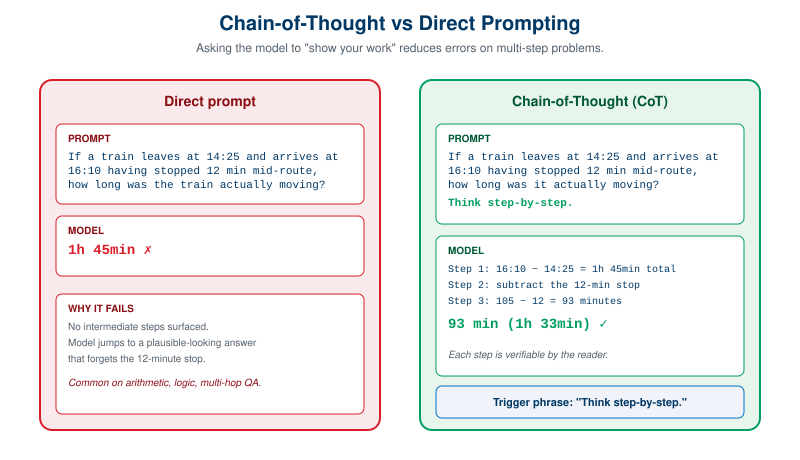
\includegraphics[width=0.95\textwidth]{assets/figures/fig10-cot-vs-direct}
\caption{Direct prompting (left) jumps to a confident wrong answer. Chain-of-Thought (right) surfaces verifiable intermediate steps.}
\label{fig:cot-vs-direct}
\end{figure}

\subsection{Zero-Shot Prompting}
You describe the task and give no examples. The model has to figure it out from its training.

\begin{examplebox}[title=\textbf{Zero-shot}]
\begin{lstlisting}[style=pythonstyle]
prompt = "Classify the sentiment of the review as POSITIVE, NEGATIVE, or NEUTRAL.\n"\
         "Review: 'Battery died after 30 minutes.'\n"\
         "Sentiment:"
\end{lstlisting}
\end{examplebox}

\textbf{When to use:} simple, well-known tasks (sentiment, easy summarisation, simple translation). Cheapest --- no examples bloat the context.

\subsection{Few-Shot Prompting}
You include 2--5 worked examples \emph{before} the new input. The model imitates the format and style.

\begin{examplebox}[title=\textbf{Few-shot}]
\begin{lstlisting}[style=pythonstyle]
prompt = """Classify each review as POSITIVE, NEGATIVE, or NEUTRAL.

Review: "Amazing camera, exceeded expectations."
Sentiment: POSITIVE

Review: "Battery dies in 30 minutes."
Sentiment: NEGATIVE

Review: "Works as described."
Sentiment: NEUTRAL

Review: "Setup was confusing but it works."
Sentiment:"""
\end{lstlisting}
\end{examplebox}

\textbf{When to use:} when zero-shot output drifts in tone, format, or label vocabulary; for unusual output schemas (custom JSON); for edge-case handling.

\examtip{If an exam scenario shows \emph{2--5 input/output pairs in the prompt}, it is few-shot. If it shows only the task description, it is zero-shot. The exam often asks ``which is the cheapest correct approach?'' --- the answer is zero-shot if the model is large/capable enough.}

\section{Designing Prompts Based on Use Case (Objective 2.2)}

\begin{figure}[h]
\centering
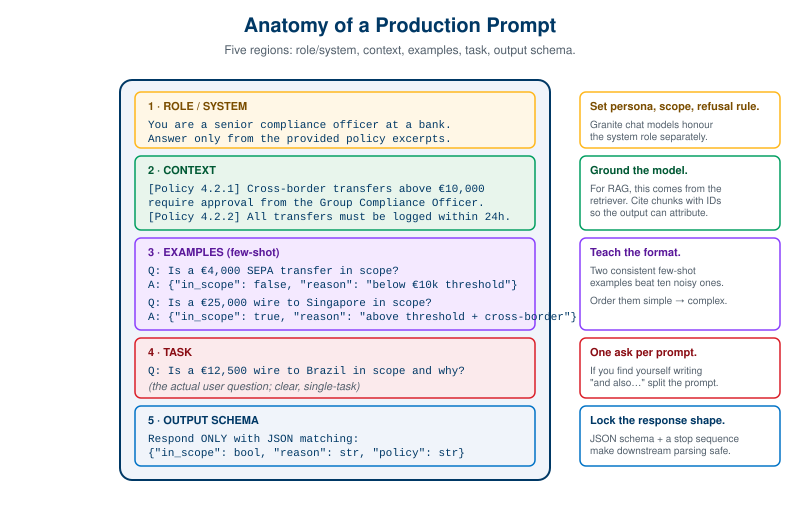
\includegraphics[width=0.95\textwidth]{assets/figures/fig08-prompt-anatomy}
\caption{The five regions of a production prompt. Most exam scenarios test whether you put the right thing in the right region.}
\label{fig:prompt-anatomy}
\end{figure}

\subsection{Match the Model to the Use Case}
You already saw the rules in Chapter~1.5. For chatty multi-turn use cases, pick an \emph{instruct} or \emph{chat} variant. For one-shot transforms, an instruct model is enough. For coding, prefer \texttt{ibm/granite-code-3-8b-instruct}.

\subsection{Conversational (Chat) Pattern}

\begin{examplebox}[title=\textbf{Chat-style prompt with system / user roles}]
\begin{lstlisting}[style=pythonstyle]
from ibm_watsonx_ai.foundation_models import ModelInference

model = ModelInference(model_id="ibm/granite-3-2-8b-instruct",
                       api_client=client,
                       params={"decoding_method": "greedy",
                               "max_new_tokens": 250,
                               "temperature": 0.3})

messages = [
    {"role": "system",
     "content": "You are a polite, concise IT helpdesk agent."},
    {"role": "user",
     "content": "My laptop won't connect to the office Wi-Fi."},
]
print(model.chat(messages=messages))
\end{lstlisting}
\end{examplebox}

\subsection{Translation Pattern}

\begin{examplebox}[title=\textbf{Translation prompt}]
\begin{lstlisting}[style=pythonstyle]
prompt = """Translate the English text into French.
Preserve technical terms and keep the same paragraph structure.

English: "Restart the router and reconnect to the corporate SSID."
French:"""
\end{lstlisting}
\end{examplebox}

\textbf{Tips:}
\begin{itemize}[leftmargin=*]
    \item Explicitly state source and target languages.
    \item Add formatting rules (preserve markdown, JSON keys, line breaks).
    \item For long content, chunk by paragraph then re-join --- avoids context-window truncation.
\end{itemize}

\section{Prompt Templates (Objective 2.3)}

\begin{keybox}
A \textbf{prompt template} is a versioned, named artefact in watsonx.ai with input variables, model binding, parameters, and (optionally) few-shot examples. Treat it like source code: store, version, deploy, monitor.
\end{keybox}

\subsection{Creating a Prompt Template Programmatically}

\begin{examplebox}[title=\textbf{Create + store a Prompt Template}]
\begin{lstlisting}[style=pythonstyle]
from ibm_watsonx_ai.foundation_models.prompts import (
    PromptTemplate, PromptTemplateManager
)
from ibm_watsonx_ai.foundation_models.utils.enums import PromptTemplateFormats

ptm = PromptTemplateManager(credentials=creds, project_id=PROJECT_ID)

template = PromptTemplate(
    name="ticket-classifier-v1",
    description="Classify support tickets into BILLING|TECH|OTHER.",
    input_variables=["ticket_text"],
    input_text=("Categorise the support ticket.\n"
                "Ticket: {ticket_text}\nCategory:"),
    examples=[
        ["My charge is wrong",   "BILLING"],
        ["The app keeps crashing", "TECH"],
    ],
    model_id="ibm/granite-3-2-8b-instruct",
    model_params={"decoding_method": "greedy",
                  "max_new_tokens": 6,
                  "stop_sequences": ["\n"]},
)
stored = ptm.store_prompt(template)
print("Asset ID:", stored.prompt_id)
\end{lstlisting}
\end{examplebox}

\subsection{Evaluating a Prompt Template}
Before promotion you should evaluate against a held-out set.

\begin{itemize}[leftmargin=*]
    \item \textbf{Metrics:} accuracy / F1 (classification), ROUGE / BLEU (summarisation, translation), exact-match (extraction).
    \item \textbf{LLM-as-judge:} a stronger model grades open-ended outputs with a rubric.
    \item \textbf{Track in governance:} attach the evaluation results to the prompt asset.
\end{itemize}

\subsection{Environment, Deployment, and Tracking}

\textbf{Environment templates} are the variations you create for dev / staging / production --- usually the same prompt text with stricter parameters or a different model. The promotion path is:

\[
\boxed{\text{Project (build)}} \;\rightarrow\; \boxed{\text{Space: Dev}} \;\rightarrow\; \boxed{\text{Space: Staging}} \;\rightarrow\; \boxed{\text{Space: Prod}}
\]

\begin{examplebox}[title=\textbf{Deploying a prompt template}]
\begin{lstlisting}[style=pythonstyle]
# Promote the asset into a deployment space
new_asset = client.repository.promote_asset(asset_id=stored.prompt_id,
                                            target_space_id=SPACE_ID)

# Create an online deployment
meta = {
    client.deployments.ConfigurationMetaNames.NAME: "ticket-classifier-prod",
    client.deployments.ConfigurationMetaNames.ONLINE: {},
    client.deployments.ConfigurationMetaNames.BASE_MODEL_ID: "ibm/granite-3-2-8b-instruct",
}
deployment = client.deployments.create(artifact_uid=new_asset["metadata"]["asset_id"],
                                       meta_props=meta)
print(client.deployments.get_id(deployment))
\end{lstlisting}
\end{examplebox}

\textbf{Tracking}: watsonx.governance automatically lineages the prompt template, its training/evaluation data, the model, the deployment, and the runtime metrics. This is your audit trail for regulated industries.

\examtip{Exam phrase to recognise: \emph{``versioned, governed, audit-friendly prompt''} $\rightarrow$ prompt \emph{template} in a deployment space, \emph{not} a free-text prompt in the SDK call.}

\section{Best Model Parameters (Objective 2.4)}

\begin{figure}[h]
\centering
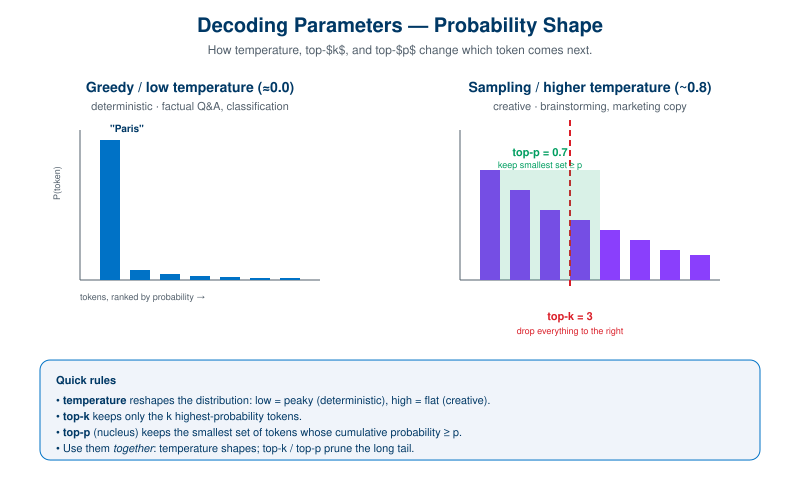
\includegraphics[width=0.95\textwidth]{assets/figures/fig09-decoding-parameters}
\caption{How temperature, top-$k$, and top-$p$ reshape the next-token distribution. Left: greedy / low temperature. Right: higher temperature with both pruning strategies applied.}
\label{fig:decoding-parameters}
\end{figure}

\subsection{Decoding Methods}

\begin{keybox}
\textbf{Decoding} = how the next token is chosen from the model's output distribution.
\begin{itemize}
    \item \textbf{Greedy decoding} --- always pick the highest-probability token. Deterministic. Best for factual / extractive tasks.
    \item \textbf{Sampling decoding} --- sample from the distribution, optionally shaped by temperature / top-k / top-p. Use for creative / diverse output.
\end{itemize}
\end{keybox}

In the watsonx API this is the \texttt{decoding\_method} parameter: \texttt{"greedy"} or \texttt{"sample"}.

\subsection{Random Seed}
When sampling, the \texttt{random\_seed} parameter makes the otherwise-random pick reproducible. Same prompt + same seed + same parameters $\Rightarrow$ same output. Useful for tests and demos.

\subsection{Repetition Penalty}
\texttt{repetition\_penalty} ($\geq 1.0$) lowers the probability of tokens that already appeared in the output. Helps prevent loops like ``thank you thank you thank you''. Typical: $1.0$--$1.2$. Above $1.5$ the model starts paraphrasing or going off-topic.

\subsection{Stopping Criteria}
The model keeps generating until one of these triggers:
\begin{itemize}[leftmargin=*]
    \item \textbf{max\_new\_tokens} --- hard ceiling on output length.
    \item \textbf{min\_new\_tokens} --- forces at least N tokens before any stop logic fires.
    \item \textbf{stop\_sequences} --- list of strings; emit one and generation stops.
    \item \textbf{time\_limit} --- maximum milliseconds of generation time per call.
    \item End-of-sequence token reached (the model's own \texttt{</s>}, \texttt{<|endoftext|>}, etc.).
\end{itemize}

\subsection{Min and Max Tokens}
\texttt{min\_new\_tokens} prevents pathological one-word answers (e.g.\ ``OK''). \texttt{max\_new\_tokens} caps cost and latency.

\begin{examplebox}[title=\textbf{Full parameter dictionary for the watsonx Text Generation API}]
\begin{lstlisting}[style=pythonstyle]
params = {
    "decoding_method":      "sample",   # or "greedy"
    "temperature":          0.7,
    "top_k":                50,
    "top_p":                0.9,
    "random_seed":          42,
    "repetition_penalty":   1.1,
    "min_new_tokens":       10,
    "max_new_tokens":       250,
    "stop_sequences":       ["\n###", "</answer>"],
    "time_limit":           20000,      # milliseconds
}
\end{lstlisting}
\end{examplebox}

\section{Benefits of Prompt Variables (Objective 2.5)}

A prompt \textbf{variable} is a placeholder in the template (\texttt{\{ticket\_text\}}, \texttt{\{language\}}, \texttt{\{tone\}}) that the application fills at call time.

\textbf{Why bother:}
\begin{itemize}[leftmargin=*]
    \item \textbf{Reusability} --- one template, many calls.
    \item \textbf{Safety} --- variables are escaped / quoted by the SDK, not concatenated by your app code. Reduces prompt-injection surface.
    \item \textbf{Governance} --- the template is a single asset to audit, instead of N free-form strings.
    \item \textbf{A/B testing} --- swap parameters or model behind the same variable contract.
\end{itemize}

\textbf{What to turn into variables:} anything that changes per request (user input, retrieved chunks, locale). Anything that stays the same (role, format rules) stays as static prompt text.

\section{Benefits of Prompt Lab (Objective 2.6)}

Prompt Lab is the no-code prompt builder inside watsonx.ai. The exam expects you to know its three editing modes:

\begin{table}[h]
\centering
\begin{tabularx}{\textwidth}{l X X}
\toprule
\textbf{Mode} & \textbf{Editor} & \textbf{Best for} \\
\midrule
\textbf{Chat}       & System + multi-turn conversation pane            & Multi-turn chat use cases \\
\textbf{Structured} & Separate fields for instruction, examples, input & Few-shot tasks, easy variable management \\
\textbf{Freeform}   & One big text box                                 & Power users, custom prompt formats \\
\bottomrule
\end{tabularx}
\caption{Prompt Lab editing modes.}
\end{table}

\textbf{Other benefits to remember:}
\begin{itemize}[leftmargin=*]
    \item Side-by-side model comparison.
    \item Live parameter sliders (temperature, top-p, max tokens).
    \item Save the prompt as a versioned template asset.
    \item One-click promotion to a deployment space.
    \item Code export (Python, curl, JS) so you can lift-and-shift into your app.
\end{itemize}

\section{Controlling Model Parameters (Objective 2.7)}

This objective overlaps with 2.4 but goes a bit deeper into \emph{shaping} the sampling distribution.

\subsection{Temperature}
Scales the logits before softmax. Higher $\Rightarrow$ flatter distribution $\Rightarrow$ more diverse / creative. Lower $\Rightarrow$ peakier $\Rightarrow$ more deterministic. Range: $0$--$2$. Greedy is equivalent to temperature $\to 0$.

\subsection{Top-K Sampling}
After computing probabilities, keep only the $k$ highest-probability tokens; renormalise; sample. Small $k$ (10--40) restricts wild outputs; large $k$ lets the rare-but-still-likely tokens through.

\subsection{Top-P Sampling (Nucleus)}
Keep the smallest set of tokens whose cumulative probability exceeds $p$; sample from that nucleus. $p=0.9$ is a popular default. More \emph{adaptive} than top-k: in confident contexts the nucleus is tiny, in ambiguous contexts it is wide.

\subsection{Random Seed and Repetition Penalty}
Already covered in 2.4. Re-flag here because the exam will recombine them.

\subsection{Stop Sequences and Token Limits}
Already covered. The official guide also explicitly mentions \emph{model generation time limit} --- the \texttt{time\_limit} parameter (milliseconds). Use it to enforce per-call SLAs.

\begin{examplebox}[title=\textbf{Symptom $\rightarrow$ parameter cheat sheet}]
\begin{lstlisting}[style=pythonstyle]
# Output is too random / off-topic
params["temperature"]  = 0.2; params["top_p"] = 0.5; params["decoding_method"] = "greedy"

# Output is too short
params["min_new_tokens"] = 50

# Output loops / repeats phrases
params["repetition_penalty"] = 1.15

# Output runs forever
params["max_new_tokens"]  = 300
params["stop_sequences"]  = ["\n\n", "###"]

# Need reproducibility for tests
params["decoding_method"] = "sample"; params["random_seed"] = 42
\end{lstlisting}
\end{examplebox}

\section{Model Risks (Objective 2.8)}

\subsection{Hallucinations}
\textbf{Underlying causes:} the model is a probabilistic next-token predictor; missing or contradictory training data; out-of-distribution prompts; high temperature.

\textbf{Techniques to avoid:}
\begin{enumerate}[leftmargin=*]
    \item Ground with \textbf{RAG} (Chapter~\ref{ch:rag}).
    \item Lower temperature, use greedy decoding for facts.
    \item Add an explicit ``I do not know'' escape hatch.
    \item Validate with a second model (LLM-as-judge) or a deterministic checker.
    \item Use Granite Guardian's groundedness check for RAG.
\end{enumerate}

\subsection{Personal Information (PII)}

\textbf{Identifying PII:} names, emails, phone numbers, government IDs, account numbers, addresses, IP addresses, dates of birth.

\textbf{Techniques for excluding PII:}
\begin{itemize}[leftmargin=*]
    \item \textbf{PII filter} on input: regex / NER pre-mask before the call. Replace the masked tokens after generation.
    \item \textbf{Granite Guardian} on output to refuse PII leakage.
    \item Do not log raw prompts; redact at the logging layer.
    \item Use a data-residency-appropriate watsonx region.
\end{itemize}

\subsection{Hate, Abuse, and Profanity (HAP)}

\textbf{HAP filter:} watsonx exposes a HAP classifier (today rolled into the Granite Guardian family) that scores text on hate / abuse / profanity. Apply on both input and output.

\subsection{Bias}
\textbf{Cause}: imbalanced training data, biased annotators, biased proxy features.

\textbf{Techniques to reduce:}
\begin{itemize}[leftmargin=*]
    \item Run demographic parity / equalised-odds tests in watsonx.governance.
    \item Add neutralising instructions in the system prompt.
    \item Use a balanced few-shot set.
    \item Document residual bias in the model card / factsheet.
\end{itemize}

\subsection{Data Bias and Poisoning}
\textbf{Data bias:} skewed training distribution leading to skewed outputs. Mitigation: curation, balanced sampling, post-hoc fairness adjustments.

\textbf{Data poisoning:} adversary injects malicious training examples. Mitigation: source provenance, signed datasets, anomaly detection on training loss, IBM Granite's documented training data and IP indemnification.

\examtip{Memorise the four risk filter families: \textbf{PII}, \textbf{HAP}, \textbf{Bias}, \textbf{Hallucination/Groundedness}. They map directly to Guardian categories and to watsonx.governance evaluators.}

\section{Putting It Together --- A Production Prompt}

\begin{examplebox}[title=\textbf{Reference production prompt skeleton}]
\begin{lstlisting}[style=pythonstyle]
SYSTEM = """You are a senior support agent at ACME Bank.
Answer ONLY from the policy excerpts in <context>.
If the answer is not in the context, reply:
  'I do not know -- please contact a human agent.'
Tone: formal, concise. Output strict JSON:
  {"answer": str, "policy_id": str | null, "confidence": "high"|"low"}"""

def build_prompt(question: str, chunks: list[str]) -> list[dict]:
    context = "\n\n".join(f"[{i+1}] {c}" for i, c in enumerate(chunks))
    return [
        {"role": "system", "content": SYSTEM},
        {"role": "user",
         "content": f"<context>\n{context}\n</context>\n\nQuestion: {question}"},
    ]

params = {
    "decoding_method":    "greedy",
    "max_new_tokens":     350,
    "temperature":        0.2,
    "stop_sequences":     ["}\n", "</answer>"],
    "time_limit":         20000,
}
\end{lstlisting}
\end{examplebox}

\section{Key Takeaways}

\begin{itemize}[leftmargin=*]
    \item \textbf{Zero-shot} = no examples; \textbf{few-shot} = 2--5 examples for tone, format, or vocabulary control.
    \item Prompt \textbf{templates} are versioned, governed, promote-able assets --- prefer them over free-text prompts in app code.
    \item Two decoding methods: \textbf{greedy} (deterministic) and \textbf{sampling} (with temperature, top-k, top-p, random\_seed).
    \item Stopping criteria: \texttt{max\_new\_tokens}, \texttt{min\_new\_tokens}, \texttt{stop\_sequences}, \texttt{time\_limit}, EOS token.
    \item Prompt Lab modes: \textbf{Chat}, \textbf{Structured}, \textbf{Freeform}.
    \item Four risk families: hallucination, PII, HAP, bias --- all mitigated via Granite Guardian + governance + good prompting.
\end{itemize}

\section{Practice Questions}

\begin{practicebox}[title=\textbf{Q2.1 --- Decoding}]
You need consistent, factual, reproducible output for an extraction task. Best decoding method?

\textbf{A.} \texttt{sample} with temperature=1.0\\
\textbf{B.} \texttt{greedy}\\
\textbf{C.} \texttt{sample} with top\_p=0.99\\
\textbf{D.} beam search with width 10

\vspace{0.2cm}\textit{Answer: B. Greedy is deterministic by definition.}
\end{practicebox}

\begin{practicebox}[title=\textbf{Q2.2 --- Parameter pick}]
The model keeps repeating the same phrase. \emph{Single} change with the biggest payoff?

\textbf{A.} Lower temperature to 0\hspace{1em}\textbf{B.} Increase \texttt{max\_new\_tokens}\\
\textbf{C.} Raise \texttt{repetition\_penalty} to $\sim$1.15\hspace{1em}\textbf{D.} Switch to a smaller model

\vspace{0.2cm}\textit{Answer: C.}
\end{practicebox}

\begin{practicebox}[title=\textbf{Q2.3 --- Stop criteria}]
You ship a chatbot and need to cap each call at 20 seconds and 300 generated tokens. Which params?

\textbf{A.} \texttt{stop\_sequences=["20s"]}\\
\textbf{B.} \texttt{max\_new\_tokens=300, time\_limit=20000}\\
\textbf{C.} \texttt{min\_new\_tokens=300, temperature=20}\\
\textbf{D.} \texttt{repetition\_penalty=20}

\vspace{0.2cm}\textit{Answer: B.}
\end{practicebox}

\begin{practicebox}[title=\textbf{Q2.4 --- Prompt template}]
You want versioning, governance, and the ability to swap models without changing app code. What do you ship?

\textbf{A.} Hard-coded f-string in your microservice\\
\textbf{B.} \texttt{PromptTemplate} stored in a watsonx project and promoted to a deployment space\\
\textbf{C.} A YAML file in your repo\\
\textbf{D.} A Jinja template on your web server

\vspace{0.2cm}\textit{Answer: B.}
\end{practicebox}

\begin{practicebox}[title=\textbf{Q2.5 --- Prompt Lab mode}]
A power user wants to hand-craft an unusual prompt with custom delimiters and no UI guardrails. Which mode?

\textbf{A.} Chat\hspace{1em}\textbf{B.} Structured\hspace{1em}\textbf{C.} Freeform\hspace{1em}\textbf{D.} JSON-only

\vspace{0.2cm}\textit{Answer: C.}
\end{practicebox}

\begin{practicebox}[title=\textbf{Q2.6 --- Risks}]
A model outputs a believable but invented case-law citation. Category?

\textbf{A.} Prompt injection\hspace{1em}\textbf{B.} Hallucination\hspace{1em}\textbf{C.} PII leak\hspace{1em}\textbf{D.} Bias

\vspace{0.2cm}\textit{Answer: B. Mitigate with RAG, low temperature, Granite Guardian groundedness check, and a citation requirement in the system prompt.}
\end{practicebox}

\begin{practicebox}[title=\textbf{Q2.7 --- HAP / PII}]
Which two filter families should you wrap around \emph{every} consumer-facing watsonx.ai endpoint?

\textbf{A.} Authentication + rate limit\\
\textbf{B.} PII + HAP via Granite Guardian\\
\textbf{C.} top\_k + top\_p\\
\textbf{D.} repetition\_penalty + min\_new\_tokens

\vspace{0.2cm}\textit{Answer: B.}
\end{practicebox}

\cleardoublepage
